% Please use the skeleton file you have received in the
% invitation-to-submit email, where your data are already
% filled in. Otherwise please make sure you insert your
% data according to the instructions in PoSauthmanual.pdf
\documentclass{PoS}
\usepackage{bm}
\usepackage{csquotes}
\usepackage{amsmath}
\usepackage{siunitx}
\usepackage{booktabs}

\title{$\bm{b}$-flavour tagging in $\bm{p\!p}$ collisions}

\ShortTitle{Flavour Tagging at LHCb}

\author{\speaker{Alex Birnkraut}\\%\thanks{A footnote may follow.}\\
        TU Dortmund\\
        E-mail: \email{a.birnkraut@cern.ch}}

%\author{Another Author\\
%        Affiliation\\
%        E-mail: \email{...}}

\abstract{In the system of neutral $B^0$ mesons $C\!P$-violating processes can be measured using time dependent analyses, as performed at the LHCb experiment. For such analyses the knowledge of the initial flavour of the mesons is mandatory. This information is provided by the Flavour Tagging, which exploits a variety of different algorithms. This article shows the good performance in different analyses which allowed high precision measurements and also the improvements which were made throughout Run I. Finally some very recent developments and new algorithms to tag the initial flavour are described.}

\FullConference{The European Physical Society Conference on High Energy Physics\\
		22--29 July 2015\\
		Vienna, Austria}


\begin{document}

\section{Introduction}\label{sec:1}

The aim of the Flavour Tagging algorithms is to determine the initial flavour of the signal $B$ meson. These algorithms are called taggers and can be classified in two groups. The so called same side (SS) taggers use charged particles which are created in the fragmentation process of the $b$ quark of the signal $B$ meson. The opposite side (OS) taggers exploit the flavour if the non-signal $b$ quark of the initial $b\bar{b}$ pair and use then the correlation at between the two flavours at production.\\
The performance of the Flavour Tagging algorihtms is characterised with the tagging efficiency
\begin{equation}
\varepsilon_\text{tag}=\frac{N_\text{right}+N_\text{wrong}}{N_\text{all}},
\end{equation}
the probability of the tagging assignment to be wrong
\begin{equation}
\omega=\frac{N_\text{wrong}}{N_\text{right}+N_\text{wrong}}
\end{equation}
and the effective tagging efficiency $\varepsilon_\text{eff}=\varepsilon_\text{tag}\left(1-2\omega\right)^2$, which indicates the statistical degradation of the information and can thus be used to compare the performance of different tagging algorithms with each other and also in different decay modes. The quantities $N_\text{wrong}$, $N_\text{right}$ and $N_\text{all}$ are the numbers of right tagged wrong tagged and all candidates. \\
In this article in section \ref{sec:2} the algorithms used at LHCb are dsecribed more in detail. The calibration of the Flavour Tagging is then explained in section \ref{sec:3}, in section \ref{sec:4} recent developments and there performance in physics analyses at LHCb from the LHC Run I are presented. Last a short conclusion will be given in section \ref{sec:conclusion}.

\section{Flavour Tagging algorithms at LHCb}\label{sec:2}

To measure time dependent flavour oscillations or $C\!P$ asymmetries  in neutral $B$ meson systems the knowledge of the $b$ quark flavour at production is mandatory. As explained in section \ref{sec:1} there are two different classes of algorithms to retain theses information: The opposite and same side taggers (Figure \ref{fig:flavtagscheme}).
\begin{figure}[htbp]
	\begin{center}
		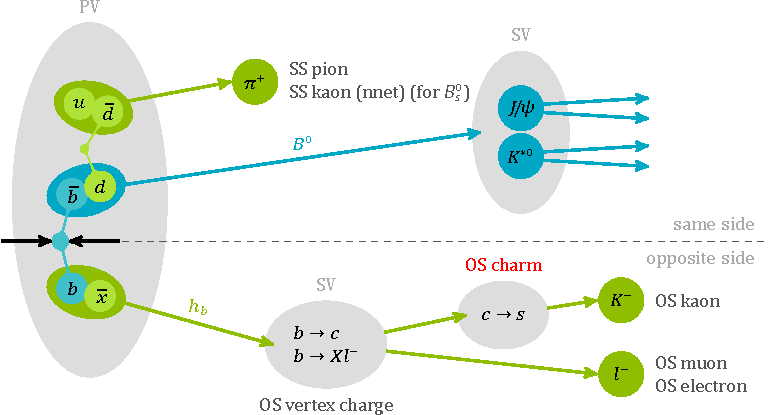
\includegraphics[width=0.68\textwidth, angle=0]{figs/FlavourTaggerScheme.pdf}
		\small{\caption{Scheme of the different flavour tagging algorithms. Same side taggers are shown in the upper part, opposite side taggers in the lower part.}}
		\label{fig:flavtagscheme}
	\end{center}
\end{figure}
Each tagger provides a decision $d$ on the initial flavour (\enquote{tag}) and a probability $\eta$ to be wrong.

\subsection{Opposite side tagging}\label{sec:OStagging}

The tagging information on the opposite side is obtained with mainly two different types of algorithms. The two lepton taggers, the OS electron and the OS muon tagger, the OS kaon and the OS charm use the charge of decay products of different decay chains of the opposite $b$ quark. All theses taggers use the charge of a single particle to provide a tag decision for the initial $b$ flavour.\\
In contrast to this method the OS vertex charge tagger does not use single tracks but a weighted charge of the whole secondary vertex to come to a tag decision. In order to do so, the secondary vertex is reconstructed first out of two tracks which have the highest probablity to originate from the $b$ hadron. After this, more tracks are added to the vertex and the weighted charge is calculated as
\begin{equation}
Q_\text{vtx}=\frac{\sum_i p_T^k(i)Q_i}{\sum_i p_T^k(i)}
\end{equation}  
The opposite side tagging is independent of the signal $B$ meson as it only investigates the propagation of the opposite $b$ quark.

\subsection{Same side tagging}

For the same side tagging one has to distinguish between $B_d^0$ and $B_s^0$ mesons as the accompanying quark is a $d$ or a $s$ quark, respectively. In case of a $B_d^0$ meson an additional $d$ quark which can hadronise with an $u$ quark into a pion emerges. Also pions from excited states as $B^*$ and $B^**$ have the same charge as pions from the direct fragmenation process with a $B$ meson. If the signal $B$ meson is a $B_s^0$ an kaon can be formed out of the additional $s$ quark and an $u$ quark. In a new development the fragmentation kaon is selected using neural nets. The so called SS kaon neural net tagger will be described more in detail in section \ref{sec:4}.

\section{Calibration of the Flavour Tagging}\label{sec:3}

The mistag estimate $\eta$ provided by the different tagging algorithms has to be corrected and transformed into the true mistag probabilty $\omega$. This is done with a linear calibration function
\begin{equation}
\omega(\eta)=p_0+p_1\left(\eta-\langle\eta\rangle\right)\label{eq:linfunc}
\end{equation}
with the mean mistag estimate $\langle\eta\rangle$. The parameters $p_0$ and $p_1$ of this calibration function are extracted in to different ways. With charged decay modes as $B^+\to J\!/\!\psi K^+$ and $B^+\to D^0\pi^+$ the true mistag $\omega$ can be extracted by comparing the tag with the charge of the kaon or pion in the final state. In neutral decay modes as $B^0\to J\!/\!\psi K^{*0}$, $B^0\to D^{*-}\mu^+\nu_\mu$ or $B_s^0\to D_s^-\pi^+$ a full time-dependent analysis is necessary to extract omega from the mixing asymmetry:
\begin{equation}
A_\text{mix}(t)\propto\left(1-2\omega\right)\cos\left(\Delta m_{d/s} t\right)
\end{equation}
In both cases the calculation of $\omega$ is done in bins of the mistag estimate $\eta$ and the linear function \ref{eq:linfunc} is fitted to the $(\omega,\eta)$ pairs. Figure \ref{fig:calibration} shows for one bin the time dependent mixing asymmetry and the linear calibration function for the calibration mode $B^0\to J\!/\!\psi K^{*0}$. 
\begin{figure}[htbp]
	\begin{center}
		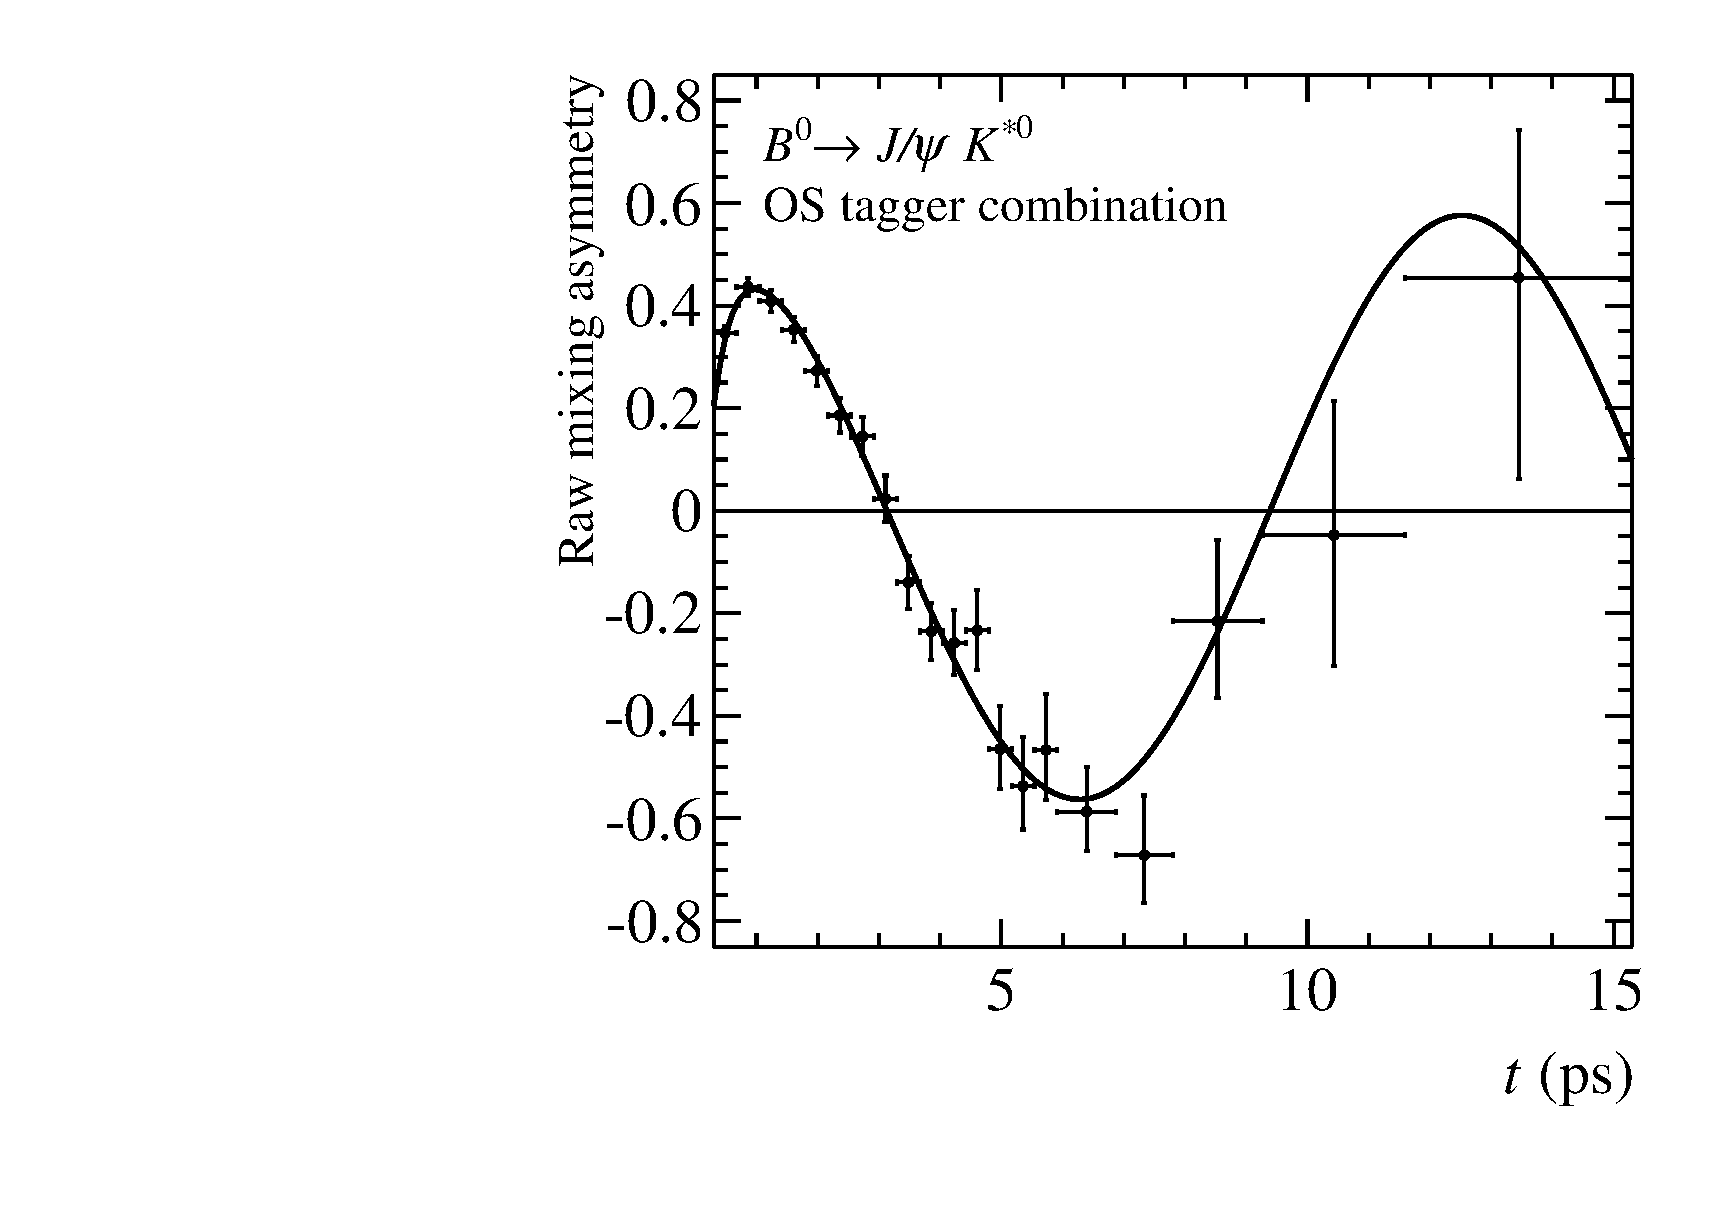
\includegraphics[width=0.34\textwidth, angle=0]{figs/KstAsym.pdf}
		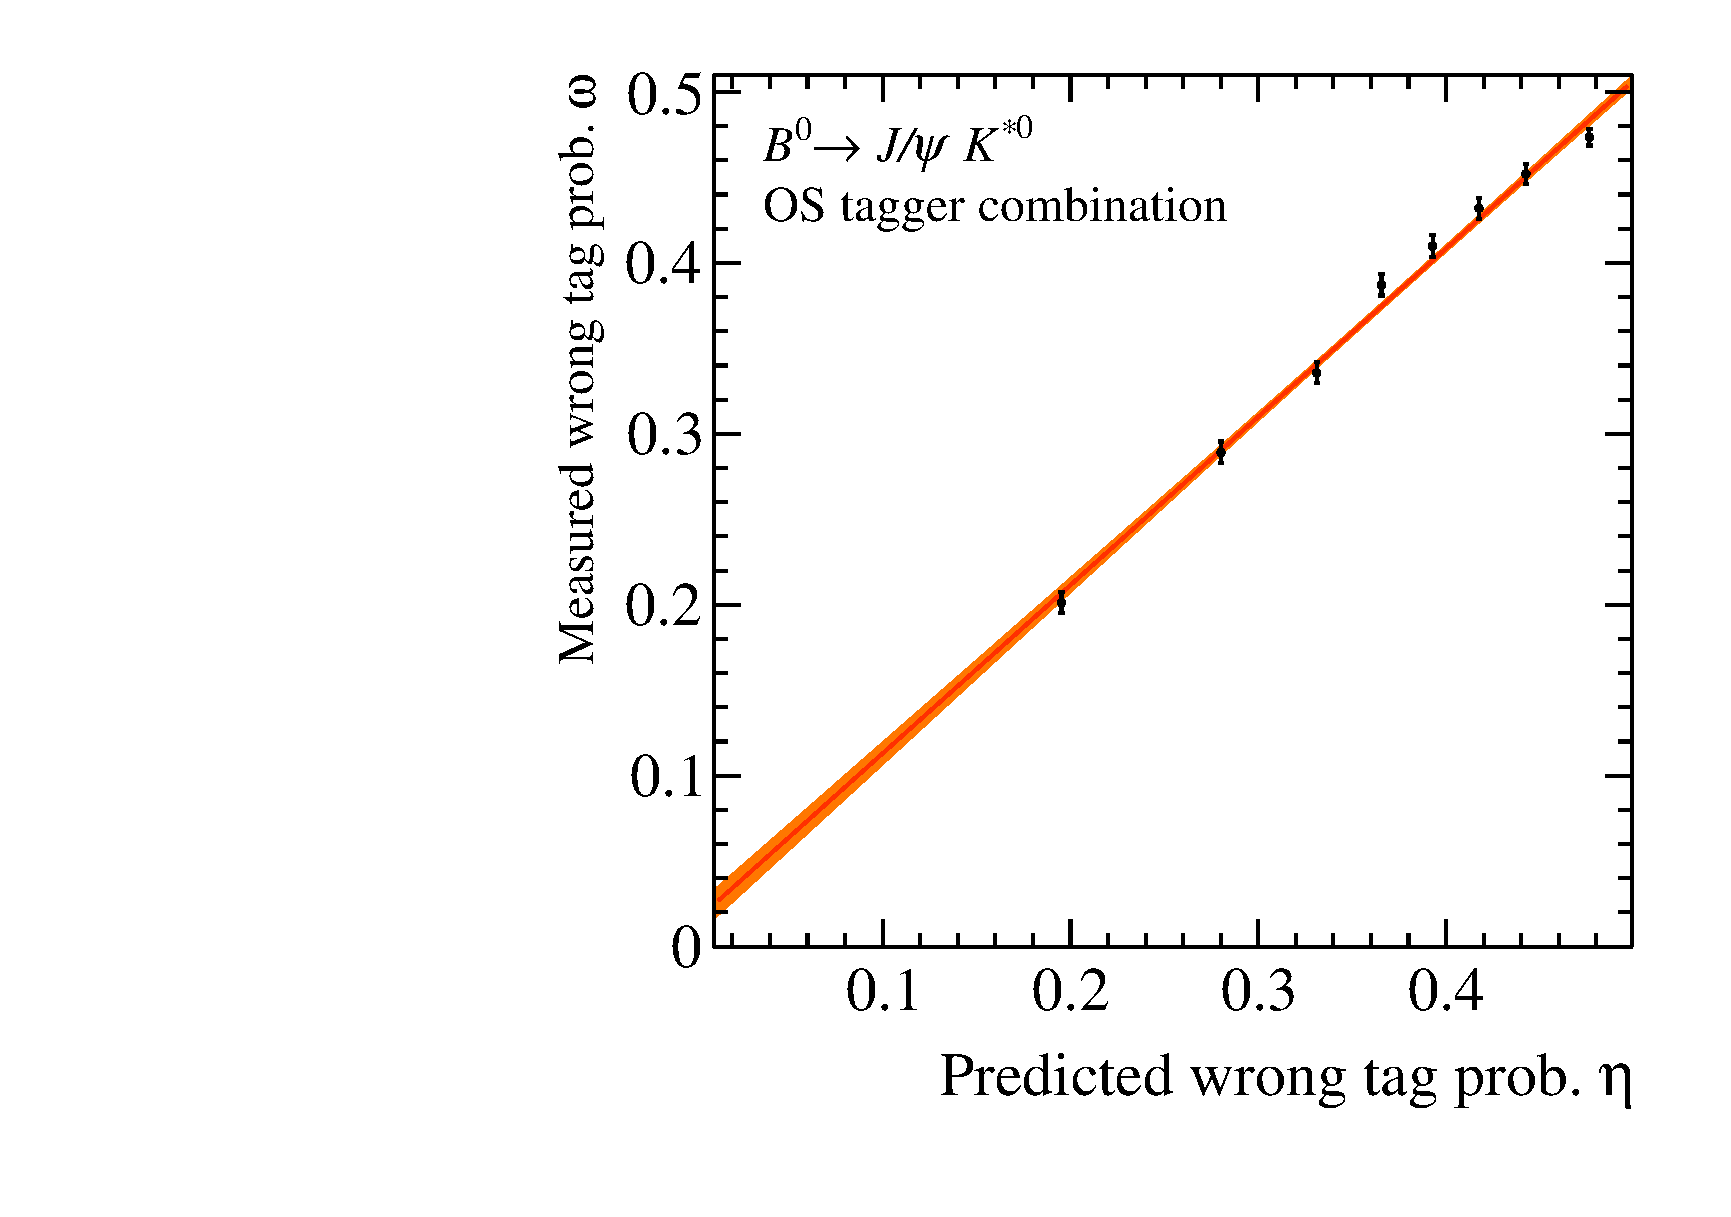
\includegraphics[width=0.34\textwidth, angle=0]{figs/Bd2JpsiKst-Kst-OST-8ScalingFunction_raw.pdf}
		\small{\caption{Mixing asymmetry (left) and calibration function (right) for the OS tagger combination in the calibration mode $B^0\to J\!/\!\psi K^{*0}$.}}
		\label{fig:calibration}
	\end{center}
\end{figure}

\section{Flavour Tagging in Run I}\label{sec:4}

For most of the analyses performed during Run I the uncertainties which came from the Flavour Tagging calibration were much smaller than the statistical uncertainties. Therefore one calibration per tagger valid for all channels was provided. The systematic uncertainties were calculated due to direct uncertainties on the calibration and the results from different control channels, which were used for the calibration. The direct uncertainties on the calibration are e.g. influences of the fit model of the mass to separete signal and background candidates.\\
For analyses where the uncertainties were dominated by the Flavour Tagging uncertainties an \enquote{ad-hoc} calibration using the best-suited control channel for the analyses were performed. \\
In the following some recent development in the Flavour Tagging are presented

\subsection{SS kaon tagging using neural nets (NN)}

The first version of the SS kaon tagger used a cut based selection to identify the tagging kaon and only to estimate the mistag probabilty $\eta$ a neural net (NN) was used. For the SS kaon neural net tagger the basid idea is to use two NN. The first NN distinguishes between the so called fragmentation tracks and the underlying event tracks (see figure \ref{fig:nnet}). The fragmentation tracks are the signal tracks for the SS kaon tagger, i.e. the tracks are the searched tagging particle tracks. 
\begin{figure}[htbp]
	\begin{center}
		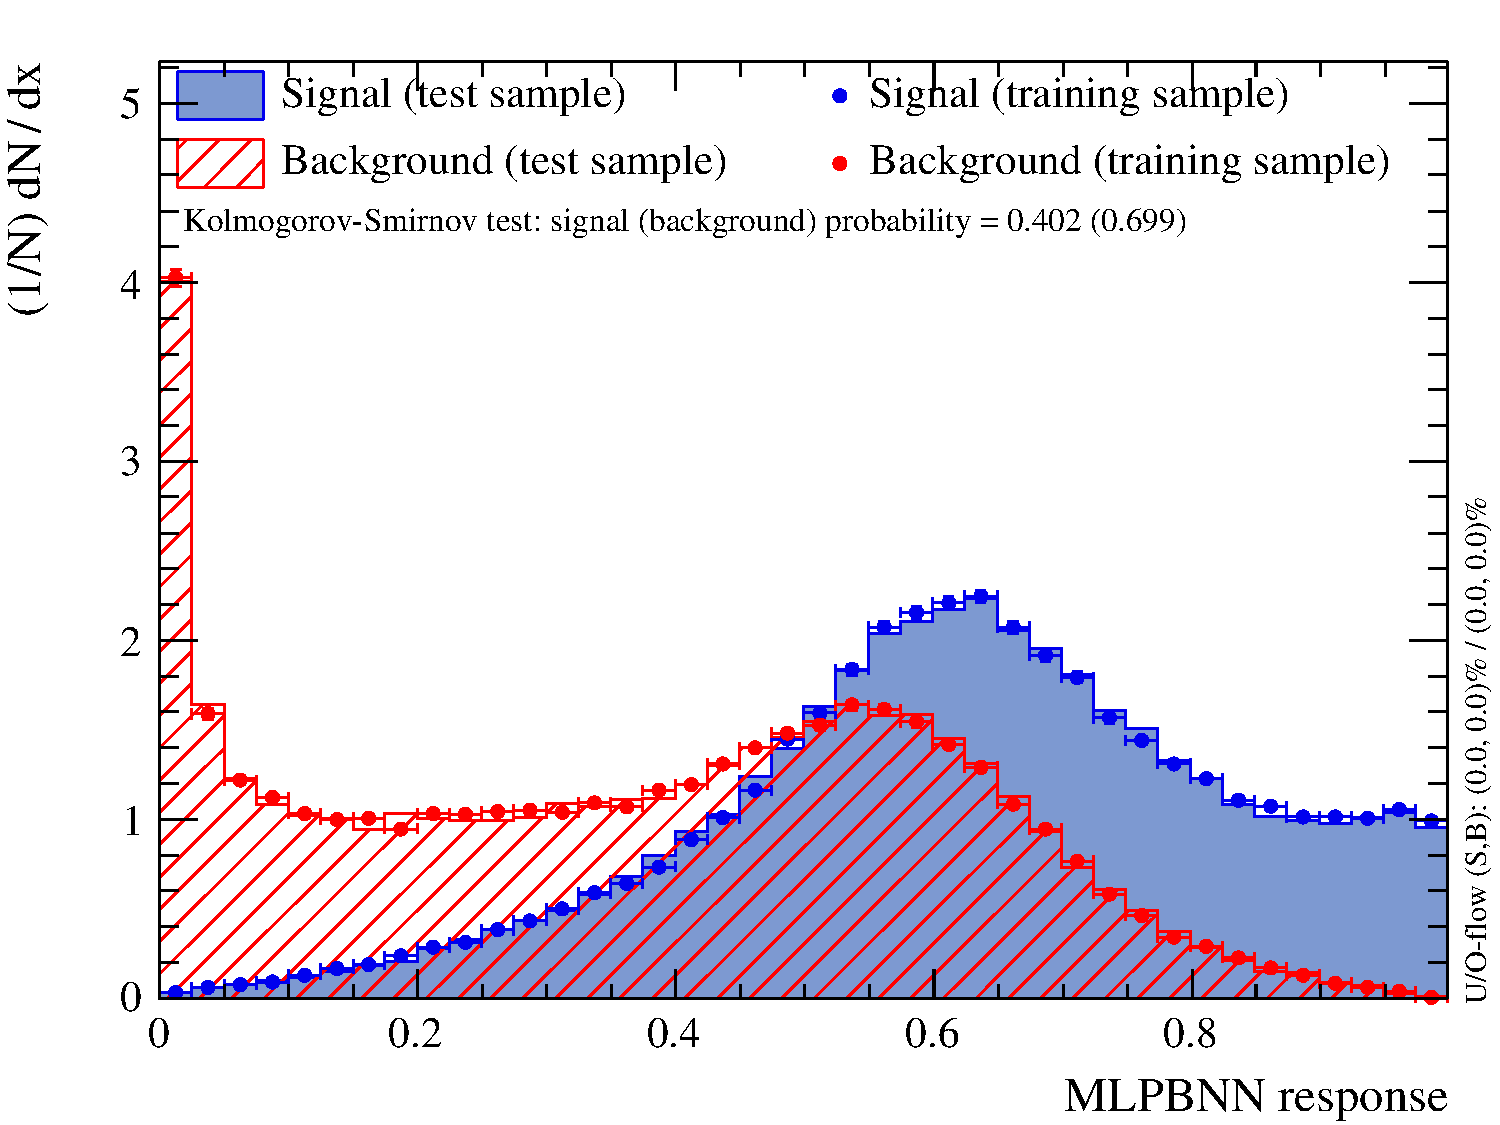
\includegraphics[width=0.58\textwidth, angle=0]{figs/sskaonNnetfirstNN3.pdf}
		\small{\caption{Neural net response for the first NN in the SS kaon tagging.}}
		\label{fig:nnet}
	\end{center}
\end{figure}
The second NN assigns the final tag and mistag based on multiple candidates.\\ 
Compared to the cut-based SS kaon the SS kaon NN gives a relative improvement of \SI{50}{\%} (\SI{41}{\%}) in $\varepsilon_\text{eff}$ for $B_s^0\to D_s^-\pi^+$ ($B_s^0\to J\!/\!\psi\phi$). This improvements can be also observed when comparing the effective tagging efficiencies in the measurements of $\phi_s$ at LHCb. The effective tagging efficiencies $\varepsilon_\text{eff}$ for the $C\!P$ analyses in \mbox{$B_s^0\to J\!/\!\psi K^+K^-$}, $\bar{B}_s^0\to J\!/\!\psi \pi^+\pi^-$ and $\bar{B}_s^0\to D_s^+D_s^-$ are listed in table \ref{tab:phis}.
\begin{table}[htbp]
  \centering
  \begin{tabular}{lcc}
  \toprule
Decay mode & $\varepsilon_\text{eff}$ (\SI{1}{fb^{-1}}) & $\varepsilon_\text{eff}$ (\SI{3}{fb^{-1}}) \\
  \midrule
  $B_s^0\to J\!/\!\psi K^+K^-$ & \SI{3.13}{\%} [3] & \SI{3.73}{\%} [4] \\ 
  $\bar{B}_s^0\to J\!/\!\psi \pi^+\pi^-$ & \SI{2.43}{\%} [5] & \SI{3.89}{\%} [6] \\
  $\bar{B}_s^0\to D_s^+D_s^-$ & - & \SI{5.33}{\%} [7] \\
  \bottomrule
  \end{tabular}
 \small{ \caption{Tagging efficiencies and effective tagging efficiencies for the $C\!P$ analyses measuring $\phi_s$. In the analyses on \SI{1}{fb^{-1}} the cut-based version of the SS kaon NN was used, the analyses on the whole Run I dataset with \SI{3}{fb^{-1}} used the neural net based version. }}
  \label{tab:phis}
\end{table} 

%\subsection{$\bm{C\!P}$ violation in $\bm{B_s^0}\bm{\to} \pmb{D_s^\mp} \pmb{K^\pm}$} 
%
%In the decay channel $B_s^0\to D_s^\mp K^\pm$ the $C\!K\!M$ angle $\gamma$ was measured in a time-dependent $C\!P$ analysis. In figure \ref{fig:DsK} the linear calibration function to transform the estimated mistag $\eta$ into the true mistag probabilty $\omega$ is shown. As already can be seen in Table \ref{tab:phis} the effective tagging efficiency is higher for decay s modes which does not contain a $J\!/\!\psi$. In $B_s^0\to D_s^\mp K^\pm$ the effective tagging efficiency for the analysis on \SI{1}{fb^{-1}} was \SI{5.07}{\%}. To this efficiency the SS kaon nnet adds more than \SI{1.3}{\%}. Finally in figure \ref{fig:DsK} the measured $C\!P$ asymmetry for one finalstate can be seen nicely.
%\begin{figure}[htbp]
%	\begin{center}
%		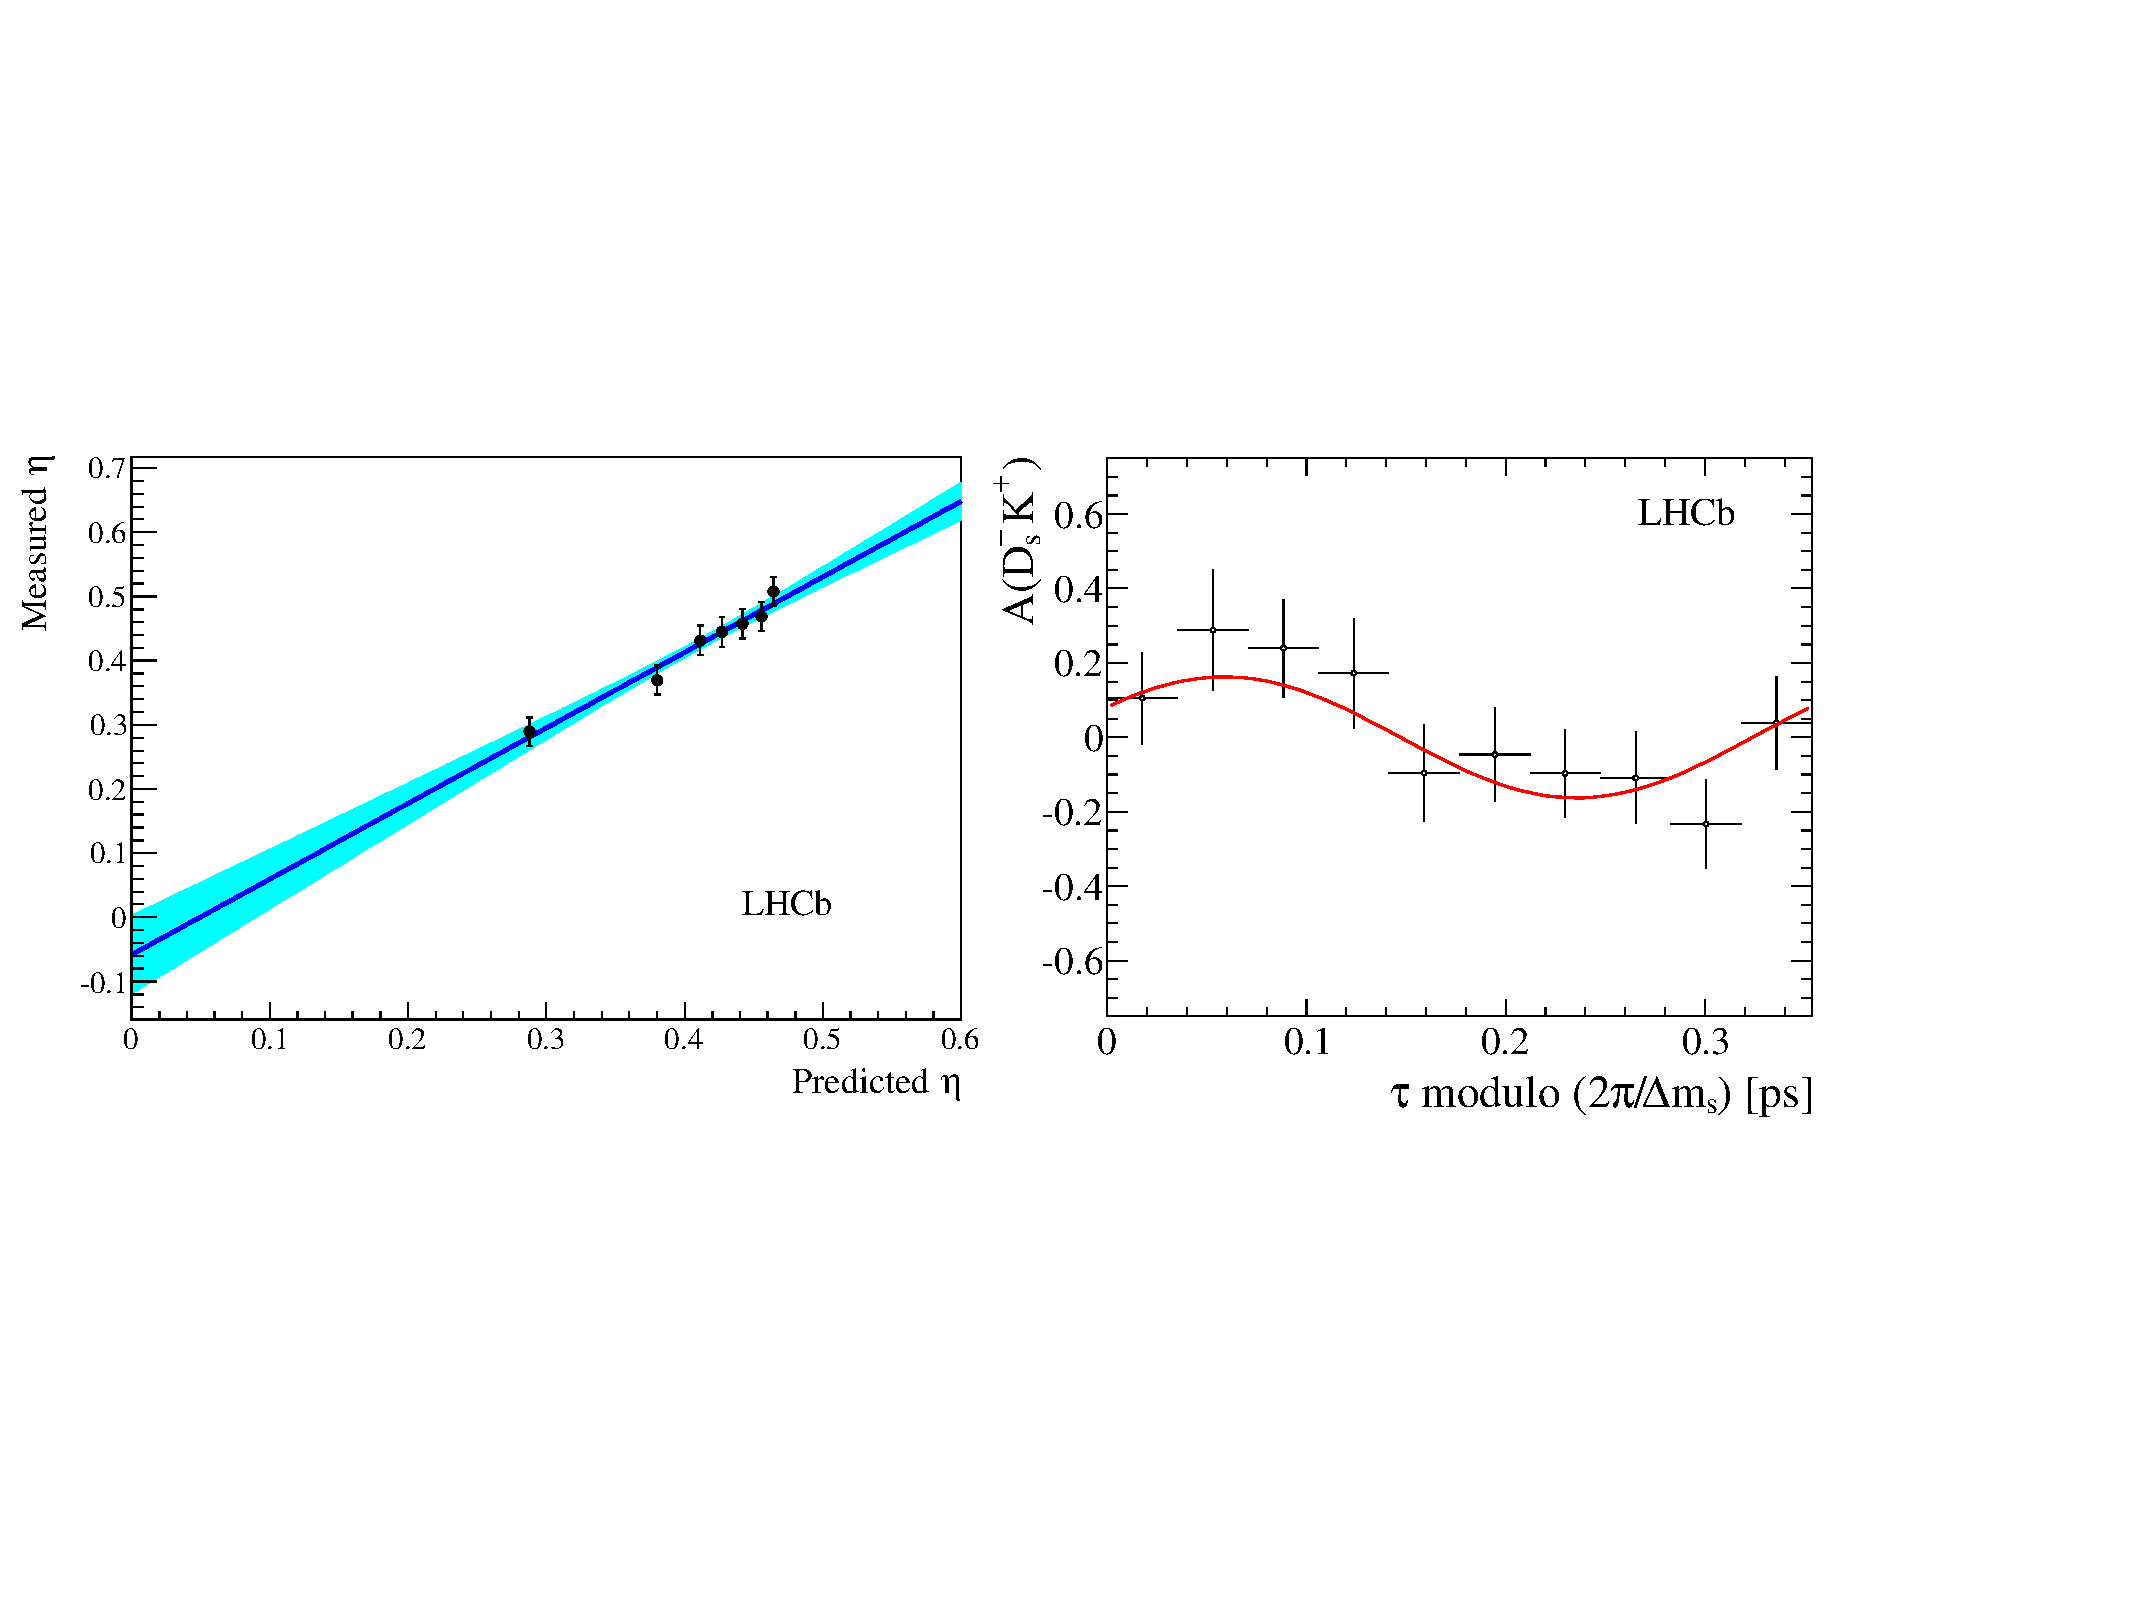
\includegraphics[width=0.8\textwidth, angle=0]{figs/CPV_DsK2.pdf}
%		\caption{Linear calibration function (left) and $C\!P$ asymmetry (right) for the measurement of the $C\!K\!M$ angle $\gamma$ in $B_s^0\to D_s^\mp K^\pm$.}
%		\label{fig:DsK}
%	\end{center}
%\end{figure}

\subsection{$\bm{C\!P}$ violation in $\bm{B^0}\bm{\to} \bm{J\!/\!\psi K_s^0}$ $\pmb{(\sin 2\beta)}$}

The measurement of $C\!P$ violation in $B^0\to J\!/\!\psi K_s^0$ was performed both on \SI{1}{fb^{-1}} and on the whole Run I dataset of \SI{3}{fb^{-1}}. The effective tagging power increased from $\varepsilon=\SI{2.38}{\%}$ (\SI{1}{fb^{-1}}) to $\varepsilon=\SI{3.02}{\%}$ (\SI{3}{fb^{-1}}). This increase was due to the usage of the SS pion tagger which adds more than \SI{0.376}{\%} in the newest analysis. As the measurement of $\sin 2\beta$ is a precision analysis an \enquote{ad-hoc} calibration was performed. The OS taggers were calibrated with the control channel $B^+\to J\!/\!\psi K^+$, the SS pion tagger was calibrated with $B^0\to J\!/\!\psi K^{*0}$. 

%\subsection{$\bm{C\!P}$ violation in $\bm{B_s^0}\bm{\to} \bm{J\!/\!\psi K_s^0}$ $\pmb{(\sin 2\beta)}$}
%
%As shown in figure \ref{fig:BsJpsi} the $B_d^0$ couldn't be excluded in the selection of $B_s^0\to J\!/\!\psi K_s^0$. Therefore the effective tagging efficiency for both modes was determined. In 
%\begin{figure}[htbp]
%	\begin{center}
%		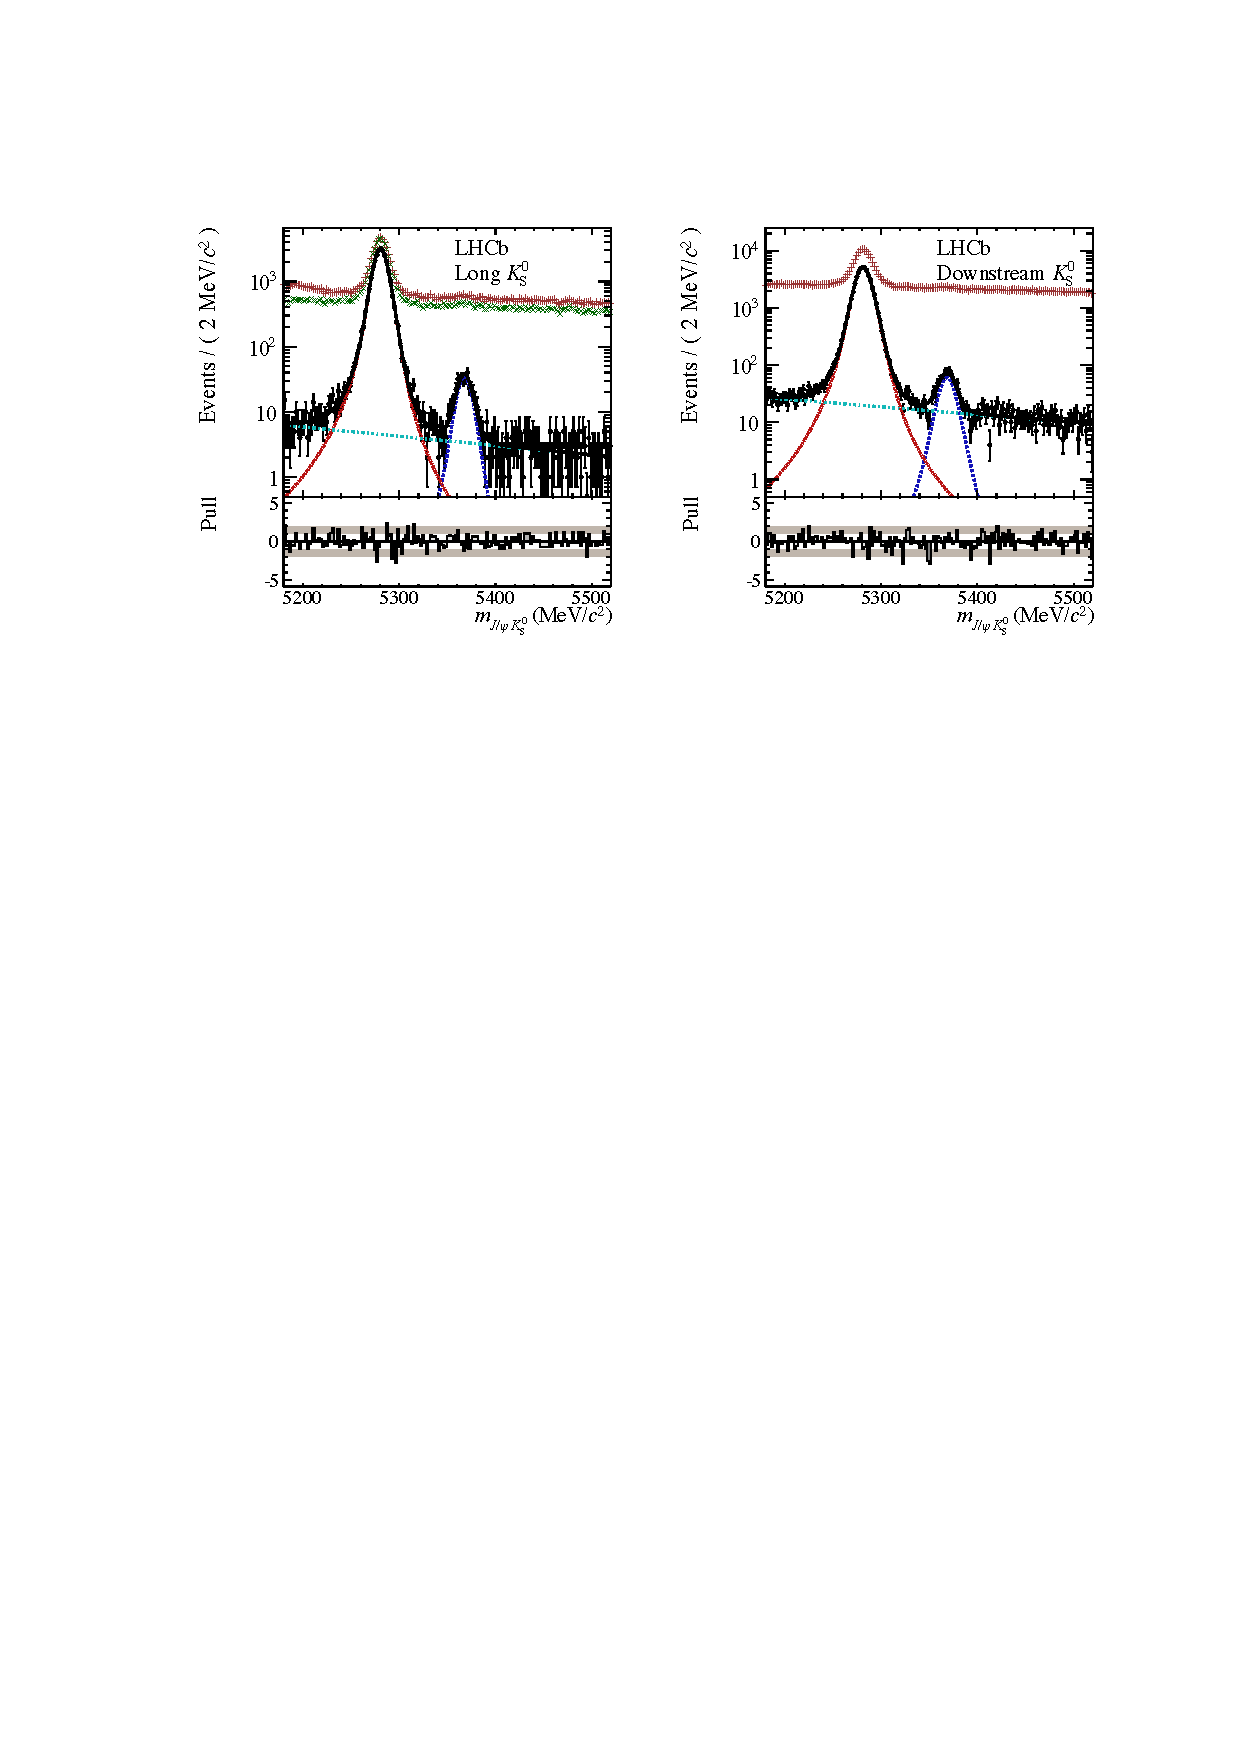
\includegraphics[width=0.8\textwidth, angle=0]{figs/CPV_BsJpsiKS.pdf}
%		\caption{Mass fit for $B_s^0\to J\!/\!\psi K_s^0$ for Longtrack (left) and Downstream (right) events.}
%		\label{fig:BsJpsi}
%	\end{center}
%\end{figure}

\subsection{OS charm tagger}

As mentioned in section \ref{sec:OStagging} the OS charm tagger uses $D$ mesons from the decay chain $b\to c$ from the opposite side $b$ quark to tag the initial flavour. The reconstructed $D$ modes related to the OS $b$ decay are listed in table \ref{tab:OScharm}.
\begin{table}[htbp]
  \centering
  \begin{tabular}{lrr}
  \toprule
  Decay mode &Relative $\varepsilon_\text{tag}$ & Relative $\varepsilon_\text{eff}$ \\
  \midrule
  $D^0\to K^-\pi^+$ & \SI{10.0}{\%} & \SI{24.0}{\%} \\ 
  $D^0\to K^-\pi^+\pi^+\pi^-$ & \SI{5.9}{\%} & \SI{8.4}{\%} \\
  $D^+\to K^-\pi^+\pi^+$ & \SI{10.3}{\%} & \SI{2.6}{\%} \\
  $D^0,D^+\to K^-\pi^+X$ & \SI{69.7}{\%} & \SI{61.5}{\%} \\
  $D^0,D^+\to K^-e^+X$ & \SI{0.5}{\%} & \SI{0.2}{\%} \\
  $D^0,D^+\to K^-\mu^+X$ & \SI{3.4}{\%} & \SI{0.3}{\%} \\
  $\Lambda_c^+\to p^+K^-\pi^+$ & \SI{0.2}{\%} & \SI{2.4}{\%} \\
  \bottomrule
  \end{tabular}
  \small{\caption{$D$ meson decay modes with their relative contributions to $\varepsilon_\text{tag}$ and $\varepsilon_\text{eff}$ which are used by the OS charm tagger.}}
  \label{tab:OScharm}
\end{table}
For each mode on boosted decision tree is used to select the $D$ candidate. The OS charm tagger provides a relatively clean measure of the $B$ flavour, e.g. it provides a low mistag probability $\eta$ and a stand-alone effective tagging efficiency of $\varepsilon_\text{eff}=\SI{0.30}{\%}$ to \SI{0.40}{\%}.

\section{Conclusion}\label{sec:conclusion}

During Run I the performance of the Flavour Tagging improved for the SS kaon tagging and for the OS tagging in the order of \SI{40}{\%} and \SI{15}{\%} respectively. Many time-dependent measurements could be performed successfully with high precision and new developments as the OS kaon NN tagging were established. 

\begin{thebibliography}{99}
\bibitem{1}LHCb Collaboration, R.Aaij et. al., {\it Opposite-side flavour tagging of $B$ mesons at the LHCb experiment, Eur.Phys.J.} C72 (2012) 2022
\bibitem{2}LHCb Collaboration, R. Aaij et. al., {\it Optimization and calibration of the same-side kaon \mbox{tagging} algorithm using hadronic $B_s^0$ decays in 2011 data,} LHCb-CONF-2012-033
\bibitem{3}LHCb Collaboration, R. Aaij et. al., {\it Measurement of $C\!P$ violation and the $B_s^0$ meson decay width difference with   $B_s^0\to J\!/\!\psi K^+K^-$ and \mbox{$\bar{B_s^0}\to J\!/\!\psi \pi^+\pi^-$} decays, } Phys.Rev. D87 (2013) 11, 112010
\bibitem{4}LHCb Collaboration, R. Aaij et. al., {\it Precision measurement of $C\!P$ violation in $B_s^0\to J\!/\!\psi K^+K^-$ decays, } Phys.Rev.Lett. 114 (2015) 4, 041801
\bibitem{5} LHCb Collaboration, R. Aaij et. al., {\it Measurement of the $C\!P$-violating phase $\phi_s$ in $\bar{B_s^0}\to J\!/\!\psi \pi^+\pi^-$ decays, } Phys.Lett. B713 (2012) 378-386
\bibitem{6} LHCb Collaboration, R. Aaij et. al., {\it Measurement of the $C\!P$-violating phase $\phi_s$ in $\bar{B_s^0}\to J\!/\!\psi \pi^+\pi^-$ decays, } Phys.Lett. B736 (2014) 186-195
\bibitem{7} LHCb Collaboration, R. Aaij et. al., {\it Measurement of the $C\!P$-violating phase $\phi_s$ in $\bar{B_s^0}\to D_s^+D_s^-$ decays, } Phys.Rev.Lett. 113 (2014) 21, 211801
\bibitem{8} LHCb Collaboration, R. Aaij et. al., {\it Measurement of $C\!P$ asymmetry in \mbox{$B_s^0\to D_s^\mp K^\pm$} decays, } JHEP 1411 (2014) 060
\bibitem{9} LHCb Collaboration, R. Aaij et. al., {\it Measurement of the time-dependent $C\!P$ asymmetry in $B^0\to J\!/\!\psi K_s^0$ decays, } Phys.Lett. B721 (2013) 24-31

\bibitem{10} LHCb Collaboration, R. Aaij et. al., {\it Measurement of $C\!P$ violation in \mbox{$B^0\to J\!/\!\psi K_s^0$} decays, } Phys.Rev.Lett. 115 (2015) 3, 031601
\bibitem{11} LHCb Collaboration, R. Aaij et. al., {\it Measurement of the time-dependent $C\!P$ asymmetries in $B_s^0\to J\!/\!\psi K_s^0$, } JHEP 1506 (2015) 131
\bibitem{12} LHCb Collaboration, R. Aaij et. al., {\it $B$ flavor tagging using reconstructed charm decays at the LHCb experiment, } LHCb-PAPER-2015.027
\bibitem{13} G. A. Krocker, {\it Development and calibration of a same side kaon tagging algorithm and measurement of the $B_s^0-\bar{B_s^0}$ oscillation frequency $\Delta m_s$ at the LHCb experiment, } PhD thesis, Heidelberg U., Sep, 2013, CERN-THESIS-2013-213

\end{thebibliography} 


\end{document}
